%===================================== CHAP 5 =================================
This section discusses the experimental procedures used to characterize semiconductor optical fibres created by the molten core fiber drawing method. Both as-drawn and laser annealed fibers are studied.  A description of sample preparation and polishing is given, followed by the methods used to create electrical contacts to fibers using lithography and physical vapor deposition. Lastly an overview of the techniques used to characterize the samples is given, including the methods of electrical measurement.

\section{Sample Preparation and Fiber Polishing}
\subsection{Overview}

\begin{figure}[]
    \centering
    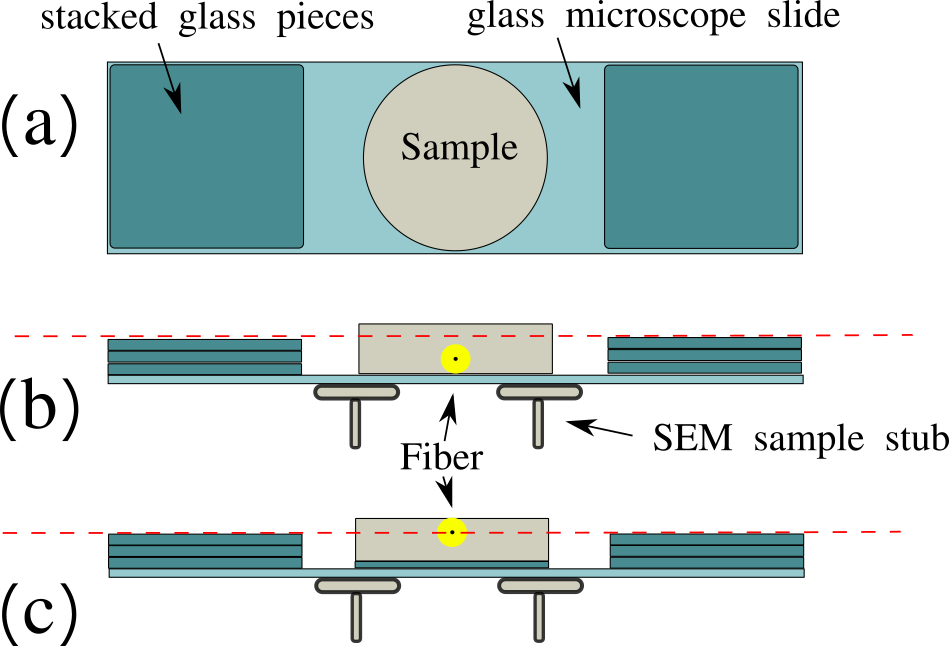
\includegraphics[width=\textwidth]{fig/Methods/polishing_jig.png}
    \caption{An illustration showing the polishing jig used to prepare fiber sample.(a) Top view of a prepared epoxy sample on the polishing jig. The sample will be polished until it meets the plane defined by the stacked glass pieces. (b) Side view of the polishing jig, where the dashed red line indicates the plane that the sample will be polished to. After polishing the epoxy sample will be plane-parallel and ready for machine polishing or further hand polishing. SEM sample stubs are used to hold the jig during polishing. (c) The sample has been flipped in order to polish to the core. Glass cover slips are chosen to match the fiber cladding thickness and placed under the sample. The polishing plane now will intersect the fiber core.}
    \label{fig:jig}
\end{figure}
  %Further if a study of the interface modifier or its diffusion into the core is required, these layers may be lost through etching. 

As the continued development of optical fibers, and fiber based devices greatly benefits from electrical characterization of the core material, the development of a sample preparation procedure is considered a major part of this work. Nearly all electrical characterization techniques, require the removal of the glass cladding to expose a section of the fiber core for electrical contacts. This is most commonly achieved by etching the fiber in Hydroflouric Acid (HF); alternatively mechanical polishing is used to remove the cladding. Previous attempts at polishing have either failed or had limited success, and no clear experimental method exists for achieving reproducible results \cite{KristinKristin_thesis_final,LapointeElectricalFibres}. 

HF has been the most common method of employed in the literature, likely due to the convenience of the approach. Hf provides a highly selective etch between Silicate glasses and Si, and thus the fiber cladding can be removed without an appreciably etch of the Si core. The rate is roughly three orders of magnitude higher for glasses than pure Si with rates on the order of $1\si{\micro\meter}$/min \cite{Liu2013UnexpectedlyAcid} and $1\si{\nano\meter}$/min \cite{Park2017AApplication} for silcate glass and c-Silicon respectively. It has also been found the HF attacks the core at grain boundaries leading to fragmentation of the core. This limits studies to single crystalline sections, introducing bias into the results  \cite{LapointeElectricalFibres}. Although HF is standard in the semiconductor industry, it is a toxic and dangerous chemical and avoiding its use is an advantage when possible \cite{Product2015SafetySheet}. Creating arrays of fibers embedded in epoxy and polishing these with established commercial processes, also shows a path towards upgrading to the commercial production of fiber based solar cells \cite{} and other devices.

\subsection{Sample Mounting and Hand Polishing}

\begin{figure}[]
    \centering
    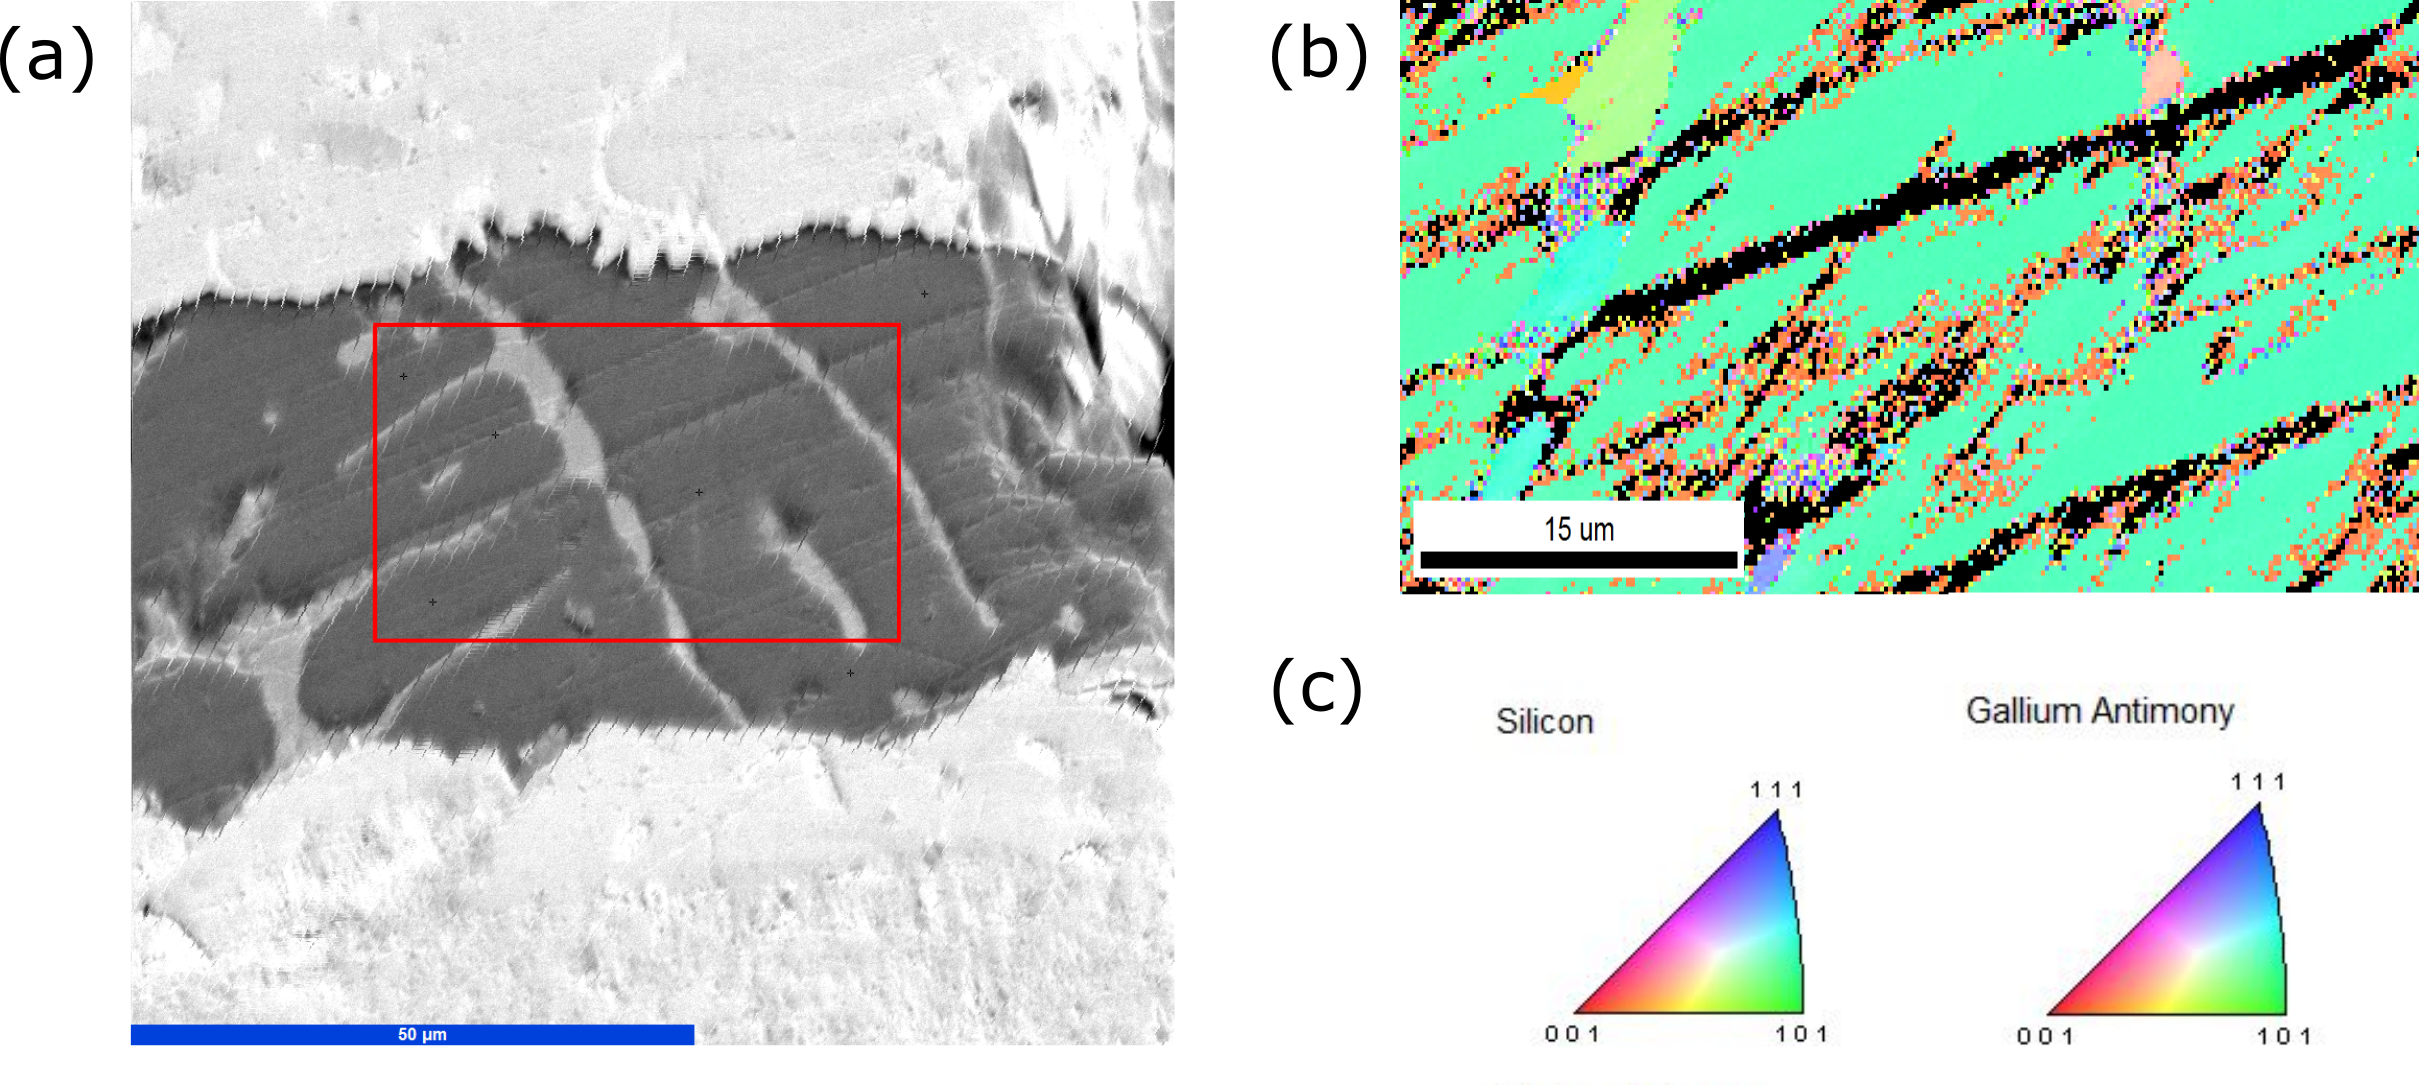
\includegraphics[width=\textwidth]{fig/ebsd.png}
    \caption{An example of a hand polished fiber illustrating how the polishing can have a large effect on the characterization of the fiber core. In this case the surface damage obscures the crystal orientation of GaSb. (a) A BSE image of a horizontal cross-section of a piece of the as-drawn Si/GaSb core fiber.  An area of interest(AOI) is marked with a red box.  (b) An EBSD mapping image of the AOI. Black lines correspond to surface damage of the fiber surface. (c) Inverse pole figures of Si and GaSb. Figure and caption adapted from \cite{Song2017Si/GaSbFiber}}
    \label{fig:ebsd}
\end{figure}
  %Further if a study of the interface modifier or its diffusion into the core is required, these layers may be lost through etching. 

Polishing of metallurgical samples for analysis is commonly achieved by mounting the specimen in epoxy, and this is the method employed in this study. Unlike bulk samples, it is necessary to polish to a fixed depth to expose a longitudinal cross section of the fiber core, which requires extra care during sample preparation. In order to obtain a cross section of the fiber core (typical dimensions: $10 - 150 \si{\micro\meter}$), the fiber must remain parallel to the polishing surface. In order to establish this plane, the fiber was first placed on a glass substrate coated in a very thin layer of silicone lubricant. A plastic mould is placed around the fiber and sealed to the substrate with a removable glue. The epoxy is poured around the fiber and cured in an oven at 65, or at room temperature. Once cured the sample is removed from the substrate and plastic mould, and is ready for polishing. 
\subsubsection{Hand Polishing Procedure}
A polishing jig made from a glass microscope slide ( see figure: ) is used to polish the backside of the sample parallel to the face. The sample is then turned over and glass cover slips of varying thickness are used to raise the sample a known distance above the plane defined by the polishing jigs bottom surface. The fiber is then polished on SiC polishing paper of varying grit to remove the cladding. The polishing process stops when the fiber is polished flush with the surfaces of the jig. The polishing process must be done very gently in order to avoid chipping or breaking the glass cladding or core. Hand polishing a fiber in this manner takes approximately two hours, as care must be taken to expose the fiber core on a fine grit paper to avoid damage. Typically a  starting grit of P1200 is used. Once the core is exposed fine polishing is done with $5 \si{\micro\meter}$, $3 \si{\micro\meter}$, and $1 \si{\micro\meter}$ grain paper. extensive care must be taken at this stage to avoid contamination. Large particles on the polishing paper will quickly ruin a sample by leaving large scratches. Even with the most care and the use of sonication to clean the sample and polishing paper, it was found that particles from the larger grit SiC paper tend to embed themselves in the epoxy and become dislodged during fine polishing to scratch the sample. 


\subsection{Machine Polishing}


As an alternative to hand polishing, machine polishing with diamond abrasive suspensions was investigated.  A struers Tegramin semiautomatic polishing machine and Struers polishing cloths were used. Polishing disks are available ranging from hard composite disks to soft cloths. Composite disks with embedded diamond are available for the roughest polishing and offers an alternative to SiC paper. These offer the advantage of reducing relief as the diamond has a high removal rate for both hard and soft materials. It also minimizes embedded abrasive particles as compared to SiC paper. For medium fine grinding of $15\si{\micro\meter}$-$9\si{\micro\meter}$ a composite disk is used with a loose diamond suspension. The diamonds embed themselves in the disk, and act similarly to a fixed abrasive. Fine polishing starting at either $9 \si{\micro\meter}$ or $3\si{\micro\meter}$ is done on polishing clothes of different resilience. A cloth of high resilience conforms less to the contours of the sample and provides less relief between hard and soft materials. A low resilience cloth provides a very gentle and fine polish, while tending to create a high relief. If necessary a final oxide polish or vibrational polish is used to produce a deformation free surface for sensitive measurements such as Electron Backscatter Diffraction (EBSD). 

During polishing both the sample holder and disk rotate. The force on the sample and the rate the diamond suspension is dispensed used are set by the user. A higher force allows for faster material removal, but can also embed particles in the sample. The principle is to use less force and less resilient cloths as the grit size is reduced to create a chip size (scratch depth) that approaches zero. While developing a new polishing process, the sample is checked frequently to determine the minimum time required to remove the scratches from the previous polishing step. 

\subsubsection{Machine Polishing Procedure}
For machine polishing samples were prepared in $\SI{2.5}{\cm}$ moulds, and the back side polished using the glass polishing jig to a thickness of $~\SI{3}{\mm}$. The sample was then glued to a cylinder of epoxy with parallel ends, to meet the height requirements of the polishing machine. Refer to appendix (A) for details on the exact polishing parameters used. The polishing depth was monitered by tracking the total sample thickness, measured with a dial indicator. The gauge is zeroed on the sample surface before polishing. Alternatively after polishing the back of the sample, the sample was reversed and the fiber polished on $\SI{15}{\micro\meter}$ and $\SI{10}{\micro\meter}$ SiC polishing paper at 150 rpm to remove the majority of the glass cladding. This method was found to leave a rougher interface between the fiber and epoxy, but greatly reduced the polishing times. 

%\begin{figure}[h!]
%    \centering
%    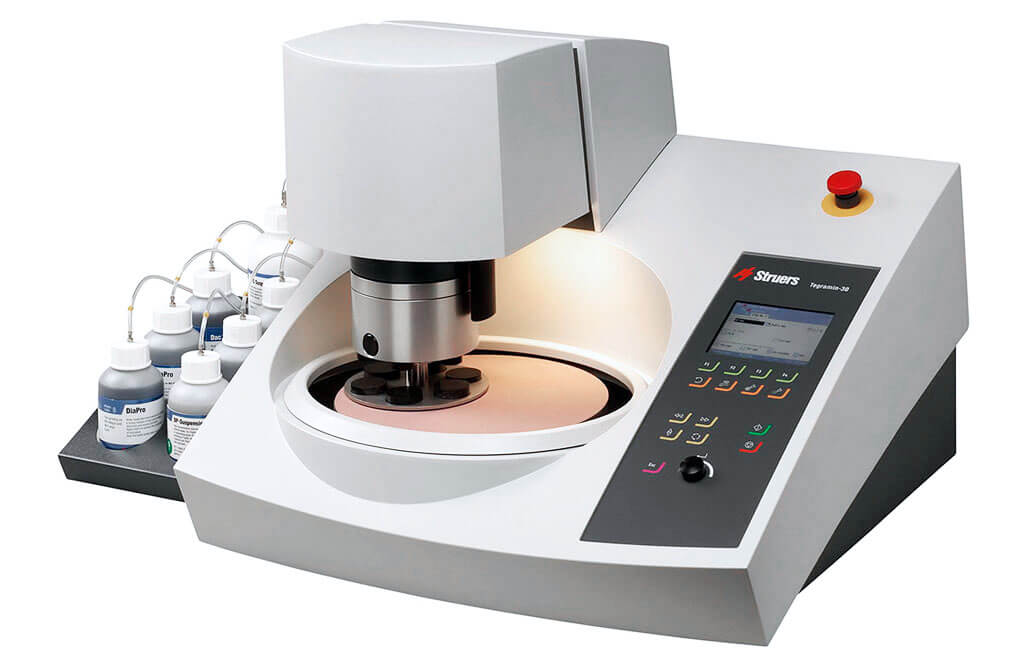
\includegraphics[width=0.5\textwidth]{fig/polishing/Tegramin.jpg}
%    \caption{Struers Tegramin polishing machine}
%   \label{fig:tegramin}
%\end{figure}

\subsection{Oven Annealing to Reduce Stresses in Fibers} \label{ovenanneal}

%Sources of Stress:
Stress is always formed in MCD fibers due to the different coefficients of thermal expansion of the core and cladding. There are further dynamics during the drawing process, including the interplay between the softening glass cladding and the expansion of the core as it solidifies that will effect the residual stresses in the fiber \cite{Healy2018AFibres}. This can lead to both tensile and compressive strain. Further annealing, after the draw, that reduces grain boundaries or transforms silicon from the amorphous to crystalline state will reduce the volume of the core and modify the stress \cite{Zhao2017EffectFibre}. This illustrates a method of controlling the stress in the fiber, and laser annealing has been used to create bandgap modification in Si \cite{Healy2014ExtremeFibres} and to directly write bragg gratings into the fiber core \cite{Fokine2017LaserFibers}. This problem has been partially addressed with the use of interface modifiers which prevent a strong bond from forming between the Si core and Si02 cladding \cite{Gibson2013AlkalineFibers}, however this has not been able to entirely eliminate the stress.. 
 Work by Zhao has shown that the stresses are concentrated in a ring near the core cladding interface \cite{Zhao2018EffectsFiber}. It was found that furnace annealing led to a reduction in stress, with greater reduction for increasing temperature. However these results should be treated carefully when comparing to our fibers as the as-drawn fibers used in this study were shown to have a low degree of crystallinity, and no interface modifier was used. The improvements in crystalinity of the core shown after the annealing process could be a factor leading to the reduction in stresses that may not be found in highly crystaline samples. However, heating the glass above the glass transition temperature and allowing for a slower cooling time then experienced in the fiber draw should have some impact on the stresses.

\begin{figure}[h]
    \centering
    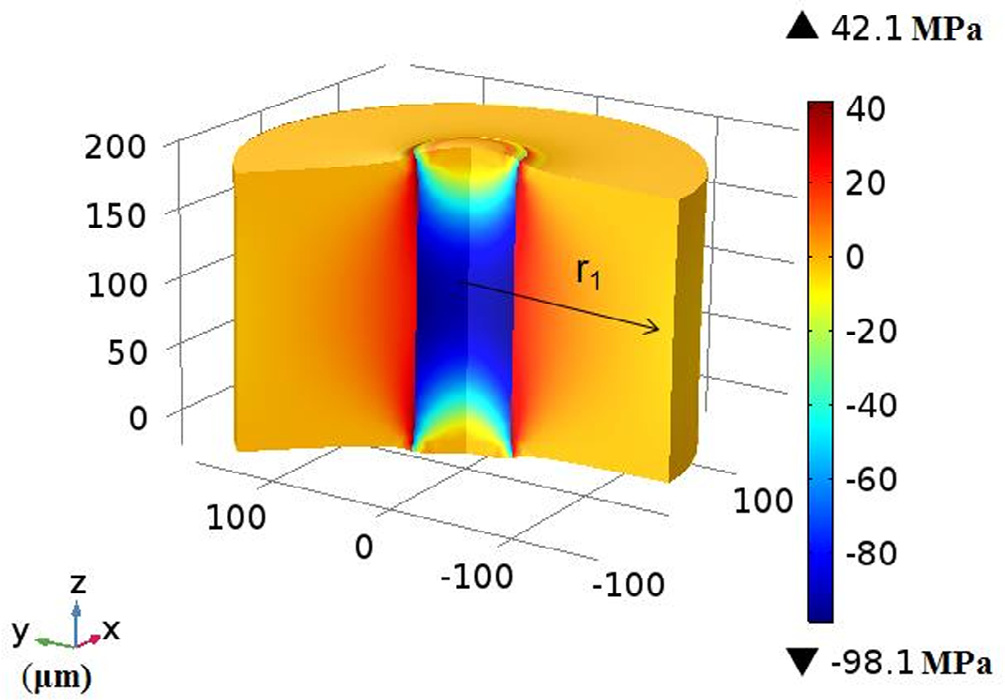
\includegraphics[width=0.5\textwidth]{fig/polishing/stress_simulation.png}
    \caption{Simulated results of stress in a Silica clad Germanium core fibre with no interface modifier, showing how stress may be distributed in a fiber. The core is $70\si{\micro\meter}$ and cladding $310\si{\micro\meter}$. Reprinted from \cite{Zhao2017EffectFiber}}
    \label{fig:my_label}
\end{figure}



\subsubsection{Oven Annealing Procedure}

To investigate the impact of furnace annealing on our samples, silicon core fibers were chosen to represent a range of core diameters and core cladding ratios. These fibers were heated in a muffle furnace to 1200 with a rate of ?, held for ? minutes and cooled with a  rate of ?. These fibers were then machine polished using diamond abrasive under the same conditions as the untreated fibers. 

To test if the polishing procedure was causing cracking, thin Si wafers (specifics) were mounted in epoxy and machine polished with the same parameters as used on the fibers. Experimentally it was not possible to polish a wafer down to fiber dimensions, but the use of large wafers would expose any significant forces involved if they were to crack during polishing.

%results: 


%Annealing, Recrystalization, core-cladding ratio. %discussion on stress observations why less in redrawn fibers, annealed fibers?


\subsubsection{Calculation of fiber Resistivity}
In order to obtain accurate resistivity results the fiber ends were polished and the core diameter was measured through a calibrated optical microscope before the fibers were mounted in epoxy. This was necessary because the fiber cross section varied slightly along the fiber, and for the case of hand drawn fibers and laser annealed fibers, this variation could be significant. The fiber chord (L in Figure \ref{fig:fiber}) was measured by optical microscope at the center of the sense contacts, after contact deposition. The contact spacing was taken as the distance between the centers of the sense contacts as defined in the contact design file. A computer program was written to calculate the sensitivity of the calculation to an error in the measured length of the chord. (appendix?)

 \cleardoublepage